\section{Introduction}

In 2003, Robert Weller (Woods Hole Oceanographic Institution [WHOI]), Albert Plueddemann (WHOI), and Roger Lukas (the University of Hawaii [UH]) proposed to establish a long-term surface mooring at the Hawaii Ocean Time-series (HOT) Station ALOHA (22°45'N, 158°W) to provide sustained, high-quality air-sea fluxes and the associated upper ocean response as a coordinated part of the HOT program, and as an element of the global array of ocean reference stations supported by the National Oceanic and Atmospheric Administration’s (NOAA) Office of Climate Observation.

With support from NOAA and the National Science Foundation (NSF), the WHOI HOT Site (WHOTS) surface mooring has been maintained at Station ALOHA since August 2004. This project aims to provide long-term, high-quality air-sea fluxes as a coordinated part of the HOT program and contribute to the goals of observing heat, freshwater, and chemical fluxes at a site representative of the oligotrophic North Pacific Ocean. The approach maintains a surface mooring outfitted for meteorological and oceanographic measurements at a site near Station ALOHA by successive mooring turnarounds. These observations are being used to investigate air-sea interaction processes related to climate variability and change.

The original mooring system is described in the mooring deployment/recovery cruise reports \parencite{Plueddemann2006, Whelan2007a}. Briefly, a Surlyn foam surface buoy is equipped with meteorological instrumentation including two complete Air-Sea Interaction Meteorological (ASIMET) systems \parencite{Hosom1995, Colbo2009} , measuring air and sea surface temperatures, relative humidity, barometric pressure, wind speed and direction, incoming shortwave and longwave radiation, and precipitation. Complete surface meteorological measurements are recorded every minute, as required to compute air-sea fluxes of heat, freshwater, and momentum. Each ASIMET system also transmits hourly averages of the surface meteorological variables via the Argos satellite system and iridium. The mooring line is instrumented to collect time series of upper ocean temperatures, salinities, and velocities with the surface forcing record. This mooring includes conductivity, salinity and temperature recorders, two Vector Measuring Current Meters (VMCMs), and two Acoustic Doppler current profilers (ADCPs). See the WHOTS-15 mooring diagram in Figure \ref{fig:whots_diagram} 

The subsurface instrumentation is located vertically to resolve the temporal variations of shear and stratification in the upper pycnocline to support the study of mixed layer entrainment. Experience with moored profiler measurements near Hawaii suggests that Richardson's number estimates over 10 m scales are adequate. Salinity is crucial to water mass stratification, as salt-stratified barrier layers are observed at HOT and in the region \parencite{Kara2000}. Thus Sea-Bird MicroCATs with vertical separation ranging from 5-20 m were used to measure temperature and salinity. A Teledyne RD Instruments (TRDI) ADCP obtains current profiles across the entrainment zone and another in the mixed layer. Both ADCPs are in an upward-looking configuration, one is at 125 m, using 4 m bins, and the other is at 47.5 m using 2 m bins. To provide near-surface velocity (where the ADCP estimates are less reliable), we deploy two VMCMs. The simple mooring design is a balance between resolving extremes versus the typical annual cycling of the mixed layer \parencite{Plueddemann2006,Santiago-Mandujano2007}.

\begin{figure}[h!]
	\begin{center}
		 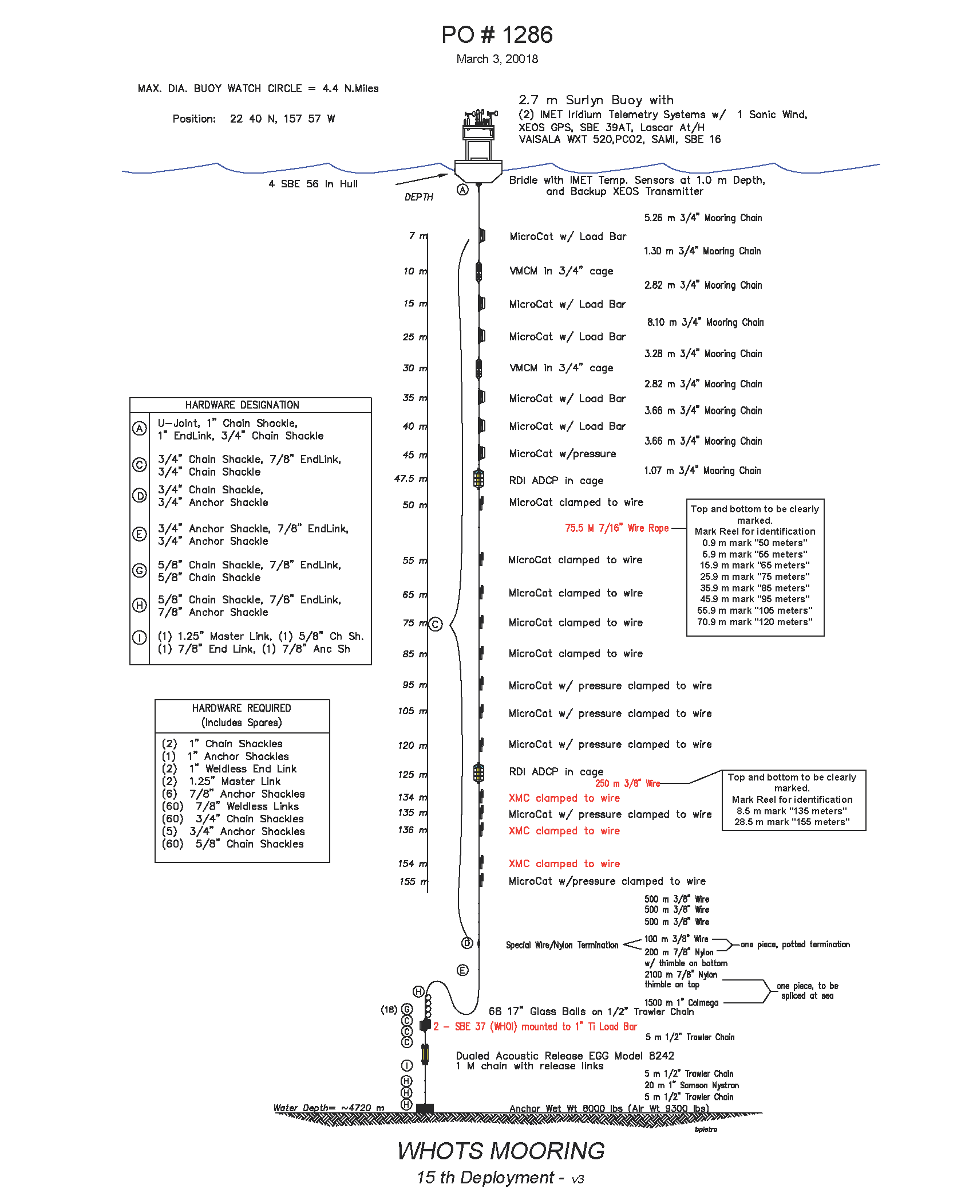
\includegraphics{2.Figures/diagram/whots_diagram.png}
		 \caption{WHOTS-15 Mooring Diagram}
		 \label{fig:whots_diagram}
	\end{center}
\end{figure}                                      

The fifteenth WHOTS mooring was deployed on March 23\textsuperscript{rd}, 2018 during an eight-day cruise (WHOTS-15 cruise) and was recovered on October 28\textsuperscript{th}, 2019 during a nine-day cruise (WHOTS-16 cruise). The cruises were aboard the NOAA Ship Hi’ialakai and Oscar Sette, respectively. A sixteenth mooring was deployed during the WHOTS-16 cruise; to be recovered in 2021.  
	
This report documents and describes the oceanographic observations made on the 15th WHOTS mooring for nearly one year and from shipboard measurements during the two cruises when the mooring was deployed and recovered. Sections II and III include a detailed description of the cruises and the mooring, respectively. Sampling and processing procedures of the hydrographic casts, thermosalinograph, and shipboard ADCP data collected during these cruises are described in Section IV. Section V includes the processing procedures for the data collected by the moored instruments: SeaCATs, MicroCATs, VMCMs, and moored ADCPs. Plots of the resulting data and preliminary analysis are presented in Section VI.

